\section{Existing \gls{bc} transducers}
One of the key factors for the purpose of this project is choosing a transducer that fits correctly with the objective pursued (testing if intelligibility can be improved with \gls{bc}. Therefore, knowledge about the available transducers at the moment is needed.The chose for a \gls{bc} require knowledge of existing \gls{bc} and vibrators of possible \gls{bc} for the purpose of this project. This section contains an analysis of the most common \gls{bc} transducers used for hearing damage assessment, as well as different kind of vibrators and actuators found during the research phase. 

\subsection{B71}
One of the most widely used \gls{bc} transducers is the Radioear Corporation B71, which belongs to the electromagnetic transducers of the variable reluctance type. The benefit of using such type of transducer is that it has a wide frequency response, high impedance and efficiency, all within a small size. The principle of the variable reluctance type is that it functions according to the horseshoe magnet principle. This principle means that there is a small air gap between the yoke, which is attached to the outer plastic cabinet of the B71, and the armature which is basically the permanent magnet \citep{the_balanced_2003}. The force in the air gap, between the yoke and the armature can be changed by generating a magnetic field in the coil, which makes the armature to move. This force changes and movements will generate vibrations corresponding to an input signal. In order to transfer acoustic signal to the skull, the transducer is required to be pressed to it with a minimum force of \SI{5}{\newton}. At hearing tests, the transducer should be pressed against the mastoid area behind the ear with the previously mentioned force. The following \autoref{fig:r_b71} shows an inside cross-section cut of the B71.

 \begin{figure}[H]
	\centering
		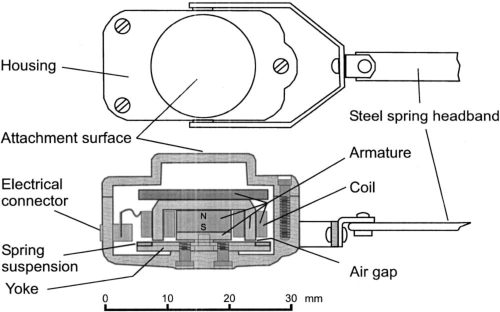
\includegraphics[width=1\textwidth]{r_b71}
		\caption{The figure shows a cross-section cut of the Radioear Corporation B71  \citep{the_balanced_2003}.}
		\label{fig:r_b71}
\end{figure}

The design of the B71 has limits which makes it not optimal for music and communications use. The transducer has high distortion in frequencies below \SI{1}{\kilo\hertz} and reaches approximately \SI{61}{\percent} distortion at \SI{250}{\hertz}. Furthermore, it has a poor frequency response. The first-order analysis of the electromagnetic circuit is explained in this article \autoref{fig:r_b71}. The conclusion for this kind of magnetic circuit is that it requires a high static magnetic force and therefore a stiff suspension to avoid the air gap collapsing. A transducer is normally designed such that its resonance frequency lays slightly above the lowest frequency in its dynamic range. With respect to the resonance formula of the circuit for B71, only the mass of the counterweight for the transducer or the stiffness for the suspension can be changed to get a better low frequency response. The formula is as following \autoref{eq:res_b71} \autoref{fig:r_b71}.

\begin{equation}\label{eq:res_b71}
f_r=\frac{1}{2 \pi \sqrt{m C}}
\end{equation}

    \startexplain
    		\explain{$f_r$ is the resonance frequency }{\si{\hertz}}
        \explain{$m$ is the mass of the counterweight}{\si{\kilo\gram}}
        \explain{$C$ is the compliance of the suspension}{\si{.(\newton\per\meter)^{-1}}}
    \stopexplain

The \autoref{eq:res_b71} explains well that either the mass or the compliance need to increase in order to achieve so. By increasing the compliance, the stiffness suffers and the air gap cannot be maintained, and therefore, only the mass can be changed. Increasing the mass of the counterweight makes the transducer bigger and also affects its weight. None of this options would correctly fit with the purpose of the transducer itself, so in order to avoid a bigger and heavier design, the Radioear Corporation B81 has been designed and will be explained next. 


\subsection{B81}
The Radioear Corporation B81 is built following the \gls{best} principle. The \gls{best} is an optimised variable reluctance type of transducer designed by the author of \citep{the_balanced_2003}. The idea of the \gls{best} principle is to cancel the static force, because then the suspension's compliance can be increased, reducing the stiffness. The benefit of this design is that the mass does not have to be increased and the distortion in the low frequency range is lowered by a factor of at least 10. It also makes the frequency response wider in the low frequency area, because the resonance frequency can be lowered with the same mass, thus avoiding the issues B71 presented. In order to accomplish this, a counterbalance for the static force has to be introduced in the system. The counterbalance is obtained by introducing a second air gap in the design. The following \autoref{fig:r_b81} shows a inside cross-section cut of the B81.

 \begin{figure}[H]
	\centering
		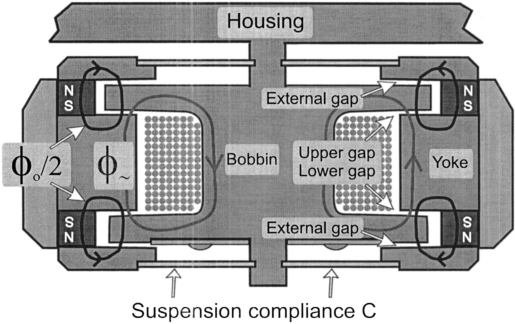
\includegraphics[width=1\textwidth]{r_b81}
		\caption{The figure shows a cross-section cut of a \gls{best} transducer. This is assumed to be very similar to the Radioear Corporation B81. Image source:  \citep{the_balanced_2003}.}
		\label{fig:r_b81}
\end{figure}

The design of the B81 transducer is a slightly modified \gls{best} transducer, adapted for \gls{bc} purposes, where an external air gap is introduced in order to stabilise the static magnetic flux and make it independent of the position of the bobbin arms in the air gaps, thus lowering the distortion.  The \gls{best} principle was originally developed for \gls{bc} implants and therefore the B81 transducer has more freedom in terms of size and power consumption. The following \autoref{fig:bc_frequency_distortion} compares the two \gls{bc} transducers mentioned so far, B71 and B81.


\begin{figure}[H]
	\centering
		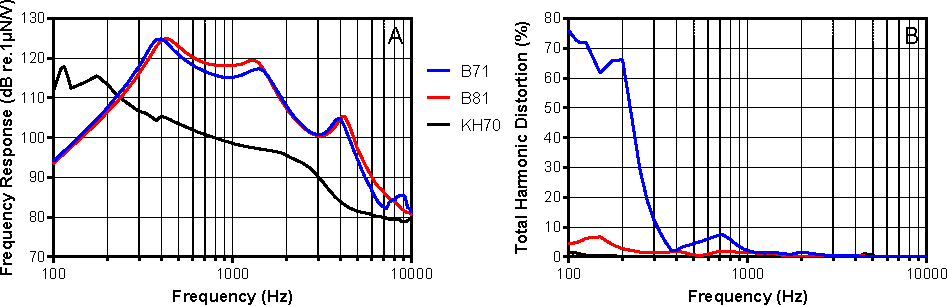
\includegraphics[width=1\textwidth]{reb_frequency_range}
		\caption{Figure A shows the frequency response for the B81 (red graph) and B71 (blue graph) transducers. Figure B shows the distortion of the  B81 (red graph) and B71 (blue graph) transducers. The other transducer (black graph), which is the \gls{bc} KH70 by Pr\"acitronic, is not considered in this project, since it is a legacy product.}
		\label{fig:bc_frequency_distortion}
\end{figure}

%\begin{figure}[H]
%\centering
%\begin{subfigure}[htbp]{0.48\textwidth}
%		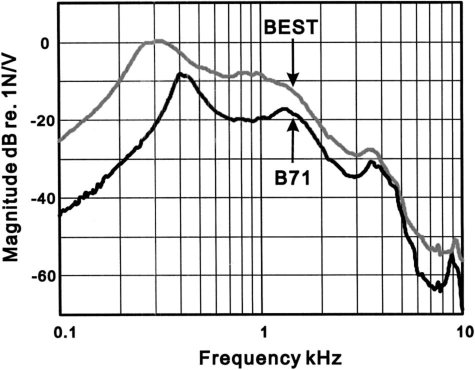
\includegraphics[width=1\textwidth]{bc_frequency_range}
%		\caption{The figure compares the frequency range for a \gls{best} and B71 transducers \citep{the_balanced_2003}.}
%		\label{fig:bc_frequency_range}
%\end{subfigure}\hspace{10pt}
%\begin{subfigure}[htbp]{0.48\textwidth}
%		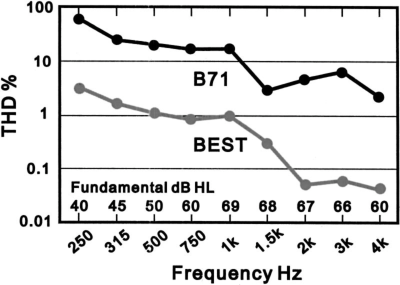
\includegraphics[width=1\textwidth]{bc_distortion}
%		\caption{The figure compares the distortion of the B81 and a \gls{best} transducers \citep{the_balanced_2003}.}
%		\label{fig:bc_distortion}
%\end{subfigure} 
%\caption{The figures display different comparisons between B71 and a \gls{best} characteristics}
%\label{fig:bc_frequency_distortion}
%\end{figure}



\autoref{fig:bc_frequency_distortion} shows that the usable frequency range for the B81 is improved compared to the B71, because the distortion is lowered significantly within the frequency area of interest, that has been specified in \autoref{speech_in_comm}. The only drawback of the B81 is, that the improvement in terms of distortion decreases towards the higher frequency range and the frequency response is not significantly improved compared to the B71. 


\section{Conclusion}

For good speech intelligibility the frequency range was found to be from \SI{355}{\hertz} up to \SI{5.68}{\kilo\hertz}  \autoref{speech_in_comm}, where the B81 suffers a bit in the frequency range from \SI{2}{\kilo\hertz} where the \si{\newton\per\volt} relation decreases more than \SI{20}{\decibel}.  The B81 transducer is a feasible choose over B71 for \gls{bc} in communications distortion-wise.







